%%%%%%%%%%%%%%%%%%%%
\chapter{Mathematical and Physical Foundations}
\label{theory}
%%%%%%%%%%%%%%%%%%%%
    \section{Stellar spectra}
    Quoting \cite{Hearnshaw2014TheStarlight}: 
    
    \noindent \guillemotleft \textit{A spectrum can be regarded as a one-dimensional image in which the intensity of light} (flux) \textit{can be analysed as a function of wavelength.} \guillemotright 

    \noindent All objects interacting electromagnetically possess a spectrum. Stellar spectra represent the energy emitted by a star at given light wavelengths. They are formed by the decomposition of the light received from the star into the different energies contained by its photons using special instruments called \textit{spectrographs} (see \textbf{Sec.} \ref{methods}.1 for a summary. Stellar spectra contain information about a star's temperature, chemical composition, intrinsic luminosity etc... With the right tools, they can also,to some extent, help understand a star's internal and orbital dynamics.
    
    \begin{figure}[H]
        \centering
        \includegraphics[width=\textwidth]{report/images/chap2_foundations/blackbody_zetgem.pdf}
        \caption{Normalised blackbody curves for temperatures between 5260-5780 [K] and wavelengths ranging from 3800-9000 \AA. }
        \label{2.1a}
    \end{figure}
    % \footnote{Proposal ID: 9786}
    \begin{figure}[H]
        \centering
        \includegraphics[width=\textwidth]{report/images/chap2_foundations/zetgem_hermes_hst.pdf}
        \caption{(top) Unprocessed merged 1D stellar spectrum of \ac{zetGem} taken by the HERMES spectrograph on the Mercator Telescope at La Palma Observatory on the 26.10.2015. The inset pictures the $H_{\alpha}$ absorption line. (bottom) Spectrum of \ac{zetGem} obtained from the \ac{STIS} instrument aboard the Hubble Space Telescope on the 26.12.2006 and retrieved from the \href{https://mast.stsci.edu/portal/Mashup/Clients/Mast/Portal.html}{MAST Archive} . Notice the resolution difference between both spectrographs and more importantly the influence of Earth's atmosphere on the general shape of HERMES spectrum and the appearance of telluric lines.}
        \label{2.1b}
    \end{figure}
    
    \section{Radial velocities}
        %say that we are looking at metallic lines.
        \begin{figure}[H]
        \centering
        \includegraphics[width=0.6\textwidth]{report/images/chap2_foundations/1280px-Proper_motion.svg.png}
        \caption{Caption}
        \label{2.2a}
        \end{figure}

        \begin{figure}[H]
        \centering
        \begin{subfigure}{.45\textwidth}
            \centering
            \includegraphics[width=\textwidth]{report/images/chap2_foundations/ccf_template.png}
        \end{subfigure}%
        \hspace{1em}
        \begin{subfigure}{.45\textwidth}
            \centering
            \includegraphics[width=\textwidth]{report/images/chap2_foundations/delCep_ccf.png}
        \end{subfigure}
        \caption{\ac{delCep}}
        \label{2.2b}
        \end{figure}

        \begin{figure}[H]
        \centering
        \includegraphics[width=0.8\textwidth]{report/images/chap2_foundations/anderson_2018.png}
        \caption{Caption}
        \label{2bonus}
        \end{figure}

        \begin{figure}[H]
        \centering
        \includegraphics[width=\textwidth]{report/images/chap2_foundations/delcep_rv.pdf}
        \caption{Caption}
        \label{2.2c}
        \end{figure}
    
    \section{Cepheids}
    
        \subsection{Stellar pulsations}
        \label{stellar_pulsations}
        %see chap 2 of anderson, talk also about the three types of cepheids + rrlyr
        \begin{figure}[H]
        \centering
        \begin{subfigure}{.45\textwidth}
            \centering
            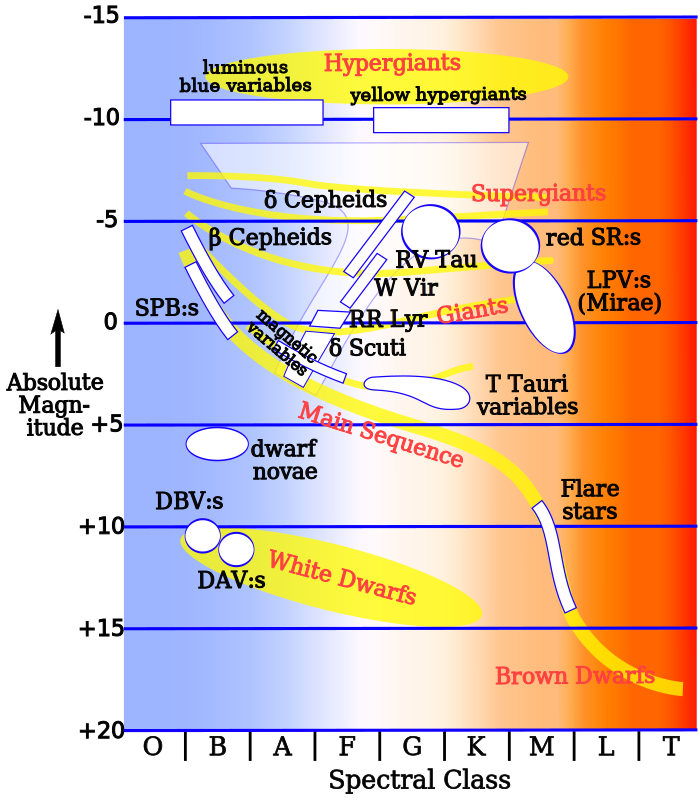
\includegraphics[width=\textwidth]{report/images/chap2_foundations/HR-vartype.png}
        \end{subfigure}%
        \hspace{1em}
        \begin{subfigure}{.45\textwidth}
            \centering
            \includegraphics[width=0.79\textwidth]{report/images/chap2_foundations/gautschy_2003.png}
        \end{subfigure}
        \caption{???}
        \label{2.3b}
        \end{figure}
        
        \begin{figure}[H]
        \centering
        \begin{subfigure}{.45\textwidth}
            \centering
            \includegraphics[width=\textwidth]{report/images/chap2_foundations/double_mode.png}
            \vspace{2em}
        \end{subfigure}%
        %\hspace{1em}
        \begin{subfigure}{.45\textwidth}
            \centering
            \includegraphics[width=\textwidth]{report/images/chap2_foundations/spherical_harmonics.png}
        \end{subfigure}
        \caption{???}
        \label{2.3c}
        \end{figure}
        
        \subsection{Cepheid binaries}
        %talk about radial velocity jitter that can be caused by companion(see candidacy exam giordano)
    \section{Finding periodicities}
    \label{finding_periods}
        \subsection{Fourier-based methods}

        
        \begin{figure}[H]
        \centering
        \begin{subfigure}{.45\textwidth}
            \centering
            \includegraphics[width=0.8\textwidth]{report/images/chap2_foundations/fourier_fit.png}
            %\vspace{2em}
        \end{subfigure}%
        \hspace{1em}
        \begin{subfigure}{.45\textwidth}
            \centering
            \includegraphics[width=\textwidth]{report/images/chap2_foundations/rcru_orbital.png}
        \end{subfigure}
        \caption{???}
        \label{2.4a}
        \end{figure}
        
            \subsubsection{The Lomb-Scargle periodogram}

            \begin{figure}[H]
            \centering
            \begin{subfigure}{.5\textwidth}
                \centering
                \includegraphics[width=0.88\textwidth]{report/images/chap2_foundations/fig01_LINEAR_data.pdf}
                \vspace{1em}
            \end{subfigure}%
            \begin{subfigure}{.5\textwidth}
                \centering
                \includegraphics[width=\textwidth]{report/images/chap2_foundations/fig14_LINEAR_window.pdf}
            \end{subfigure}
            \begin{subfigure}{\textwidth}
                \centering
                \includegraphics[width=\textwidth]{report/images/chap2_foundations/fig02_LINEAR_PSD.pdf}
                %\vspace{2em}
            \end{subfigure}%
            \caption{???}
            \label{2.4b}
            \end{figure}
            
        \subsection{Other methods}

        
    \section{Distance correlation-based periodograms}

    
        \begin{figure}[H]
        \centering
        \includegraphics[width=0.5\textwidth]{report/images/chap2_foundations/carolo_2014.png}
        \caption{Caption}
        \label{2.5a}
        \end{figure}
        
        \subsection{Mathematical framework}

                
        \begin{figure}[H]
        \centering
        \begin{subfigure}{.45\textwidth}
            \centering
            \includegraphics[width=\textwidth]{report/images/chap2_foundations/Correlation_examples2.svg.png}
            \vspace{1em}
        \end{subfigure}%
        \hspace{1em}
        \begin{subfigure}{.45\textwidth}
            \centering
            \includegraphics[width=\textwidth]{report/images/chap2_foundations/Distance_Correlation_Examples.svg.png}
        \end{subfigure}
        \caption{???}
        \label{2.5b}
        \end{figure}

        \subsection{A didactic example}

        \begin{figure}[H]
        \centering
        \includegraphics[width=\textwidth]{report/images/chap2_foundations/Smus.png}
        \caption{Caption}
        \label{2.5c}
        \end{figure}

        \begin{figure}[H]
        \centering
        \includegraphics[width=\textwidth]{report/images/chap2_foundations/betador.png}
        \caption{Caption}
        \label{2.5d}
        \end{figure}